\section{Visualisation}
\subsection{Overview} [talk about the features of the tool here]
\begin{figure}[H]
     \centering
     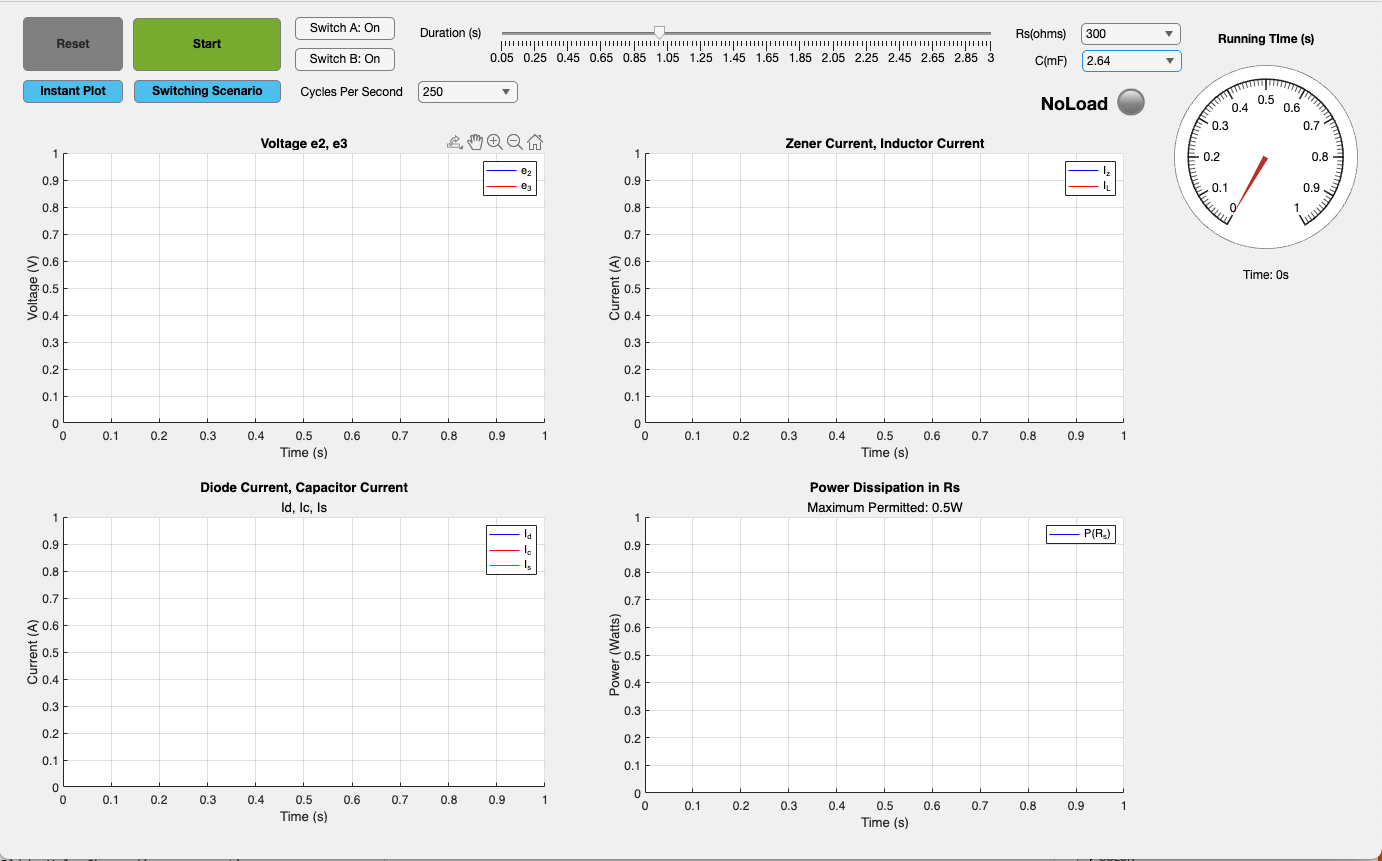
\includegraphics[width=\textwidth]{graphics/visualisation/inactive_ui}
     \caption{User interface of the visualisation while it is inactive}
\end{figure}

\subsubsection{Implementation}
The visualisation tool as implemented using MATLAB AppDesigner. [continue]

\pagebreak
\subsection{Usage Guide}
\subsubsection{Buttons}
\begin{figure}[H]
     \centering
     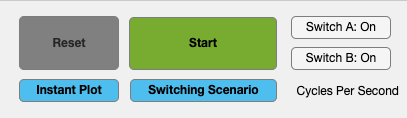
\includegraphics[width=10cm]{graphics/visualisation/ui_buttons}
     \caption{Buttons used in the visualisation interface}
\end{figure}

\paragraph{Switch Buttons}
\begin{itemize}
	\item The "Switch A" and "Switch B" buttons are used to turn on/off the primary and secondary switches in the multi-mode load respectively
	\item Pressing the button once will activate the switch.
	\item Once activated, pressing again will deactivate the switch.
	\item The combination of the switch states is used to determine the mode of operation.
\end{itemize}

\paragraph{Reset} The reset button is used to reset the simulation state. When it is pressed, the user is presented a dialog that the simulation has been reset. 
\begin{figure}[H]
     \centering
     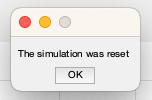
\includegraphics[width=5cm]{graphics/visualisation/dialog_reset}
     \caption{Dialog showing the user that the simulation has been reset}
\end{figure}
Resetting the simulation involves,
\begin{itemize}
	\item Clearing the graphs
	\item Resetting the RK4 initial values
	\item Resetting the time index
	\item Resetting the UI state
\end{itemize}

\paragraph{Start} The start button is used to start the simulation. When it is pressed, the program will begin to solve and plot the differential equations of the system, using RK4 over the specified duration and time step.
When the simulation is active,
\begin{itemize}
	\item The start button changes appearance to a pause button which can be used to stop, and later, resume the simulation
\begin{figure}[H]
     \centering
     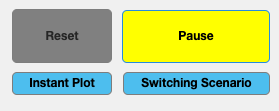
\includegraphics[width=10cm]{graphics/visualisation/pause_button}
     \caption{Dialog showing the user that the simulation has been reset}
\end{figure}
	\item The indicator is updated with a green light to show the simulation is running. The current mode of operation (determined by the switch buttons) is shown in the indicator.
\begin{figure}[H]
     \centering
     \begin{subfigure}[b]{0.45\textwidth}
         \centering
    	 
\includegraphics[width=2.5cm]{graphics/visualisation/ui_indicator_load}
     	\caption{Status indicator of the simulation while it is inactive under no load conditions}
     \end{subfigure}
     \hfill
     \begin{subfigure}[b]{0.45\textwidth}
         \centering
    	 
\includegraphics[width=3.5cm]{graphics/visualisation/ui_indicator_load_active}
     	\caption{Status indicator of the simulation while it is active under an inductive load}
     \end{subfigure}
     \hfill
\end{figure}
\end{itemize}

\pagebreak
\paragraph{Instant Plot} [description of feature]
\begin{figure}[H]
     \centering
     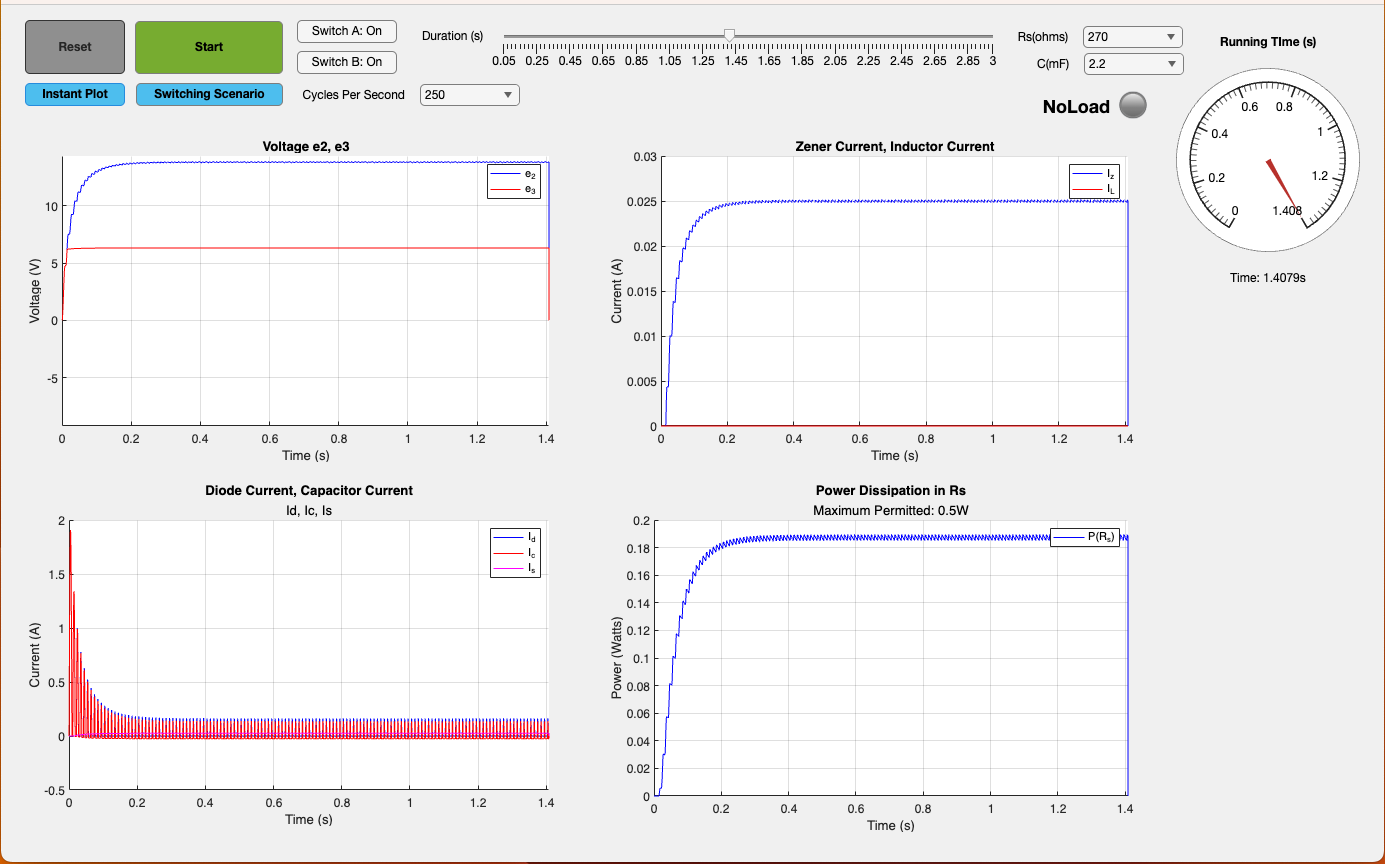
\includegraphics[width=\textwidth]{graphics/visualisation/no_load_instant_plot}
     \caption{The visualisation after pressing the Instant Plot button with no load conditions}
\end{figure}

\paragraph{Switching Scenario} [description of feature]
\begin{figure}[H]
   \centering
   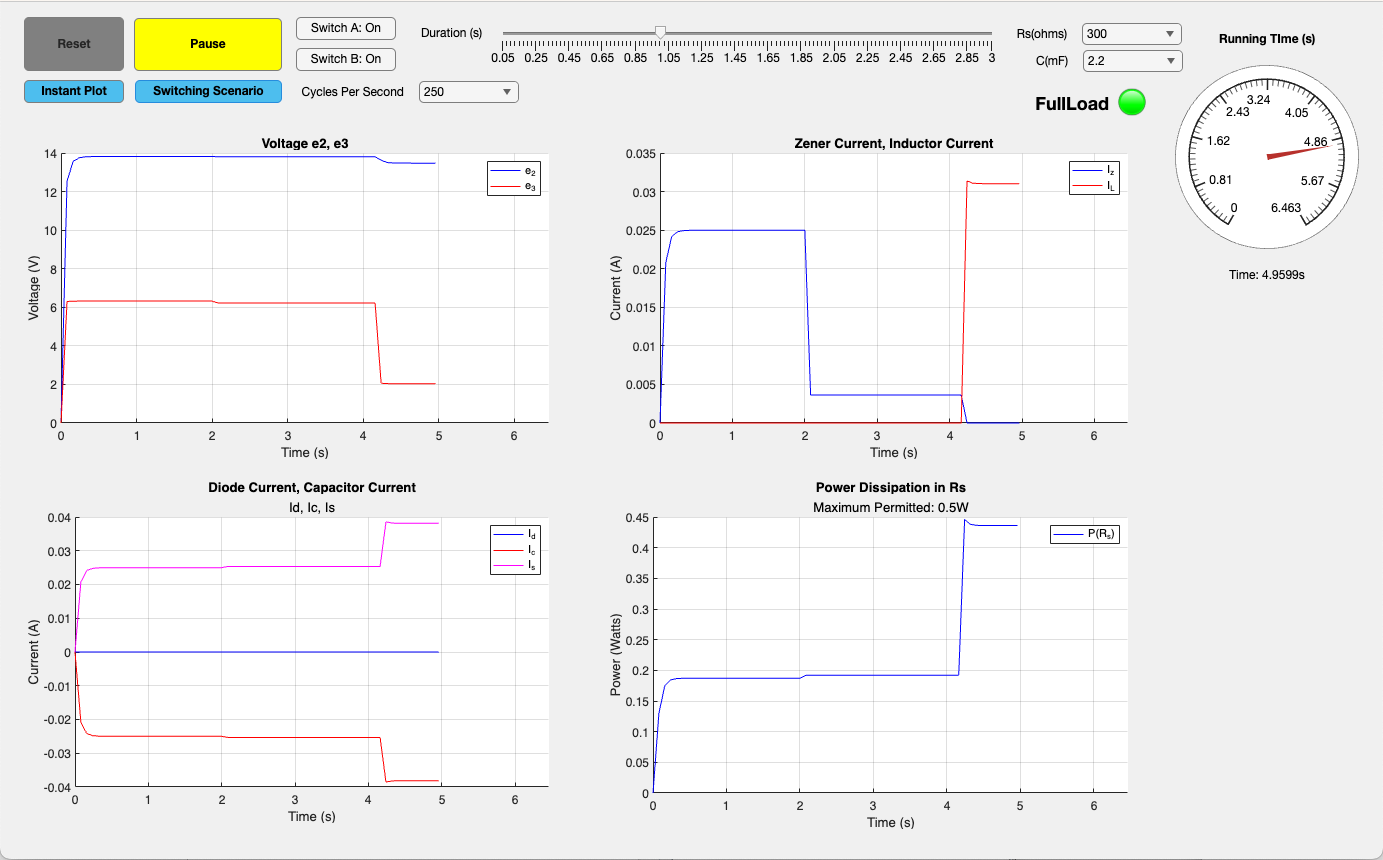
\includegraphics[width=\textwidth]{graphics/visualisation/switching_3}
   \caption{The visualisation a few seconds after pressing the Switching Scenario button}
\end{figure}

\subsubsection{Dropdowns}
\begin{figure}[H]
     \centering
     \begin{subfigure}[b]{0.3\textwidth}
         \centering
    	 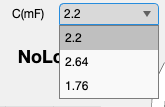
\includegraphics[width=\textwidth]{graphics/visualisation/ui_dropdowns_C}
     	\caption{Dropdown used to control the capacitance $C$ value}
     \end{subfigure}
     \hfill
     \begin{subfigure}[b]{0.3\textwidth}
         \centering
    	 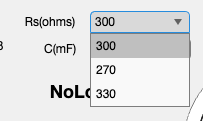
\includegraphics[width=\textwidth]{graphics/visualisation/ui_dropdowns_Rs}
     	\caption{Dropdown used to control the resistance $R_s$ value}
     \end{subfigure}
     \hfill
     \begin{subfigure}[b]{0.3\textwidth}
         \centering
    	 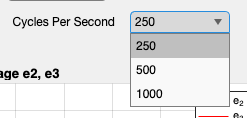
\includegraphics[width=\textwidth]{graphics/visualisation/ui_dropdowns_cycles}
     	\caption{Dropdown used to control the sampling rate $c$. Time step $h$ is determined using $\frac{T}{c}$}
     \end{subfigure}
     \hfill
\end{figure}
These values cannot be modified during the simulation. Doing so will result in the simulation being reset and the user must run the simulation again. A prompt will be shown if a change is detected while the simulation is active.
\begin{figure}[H]
     \centering
     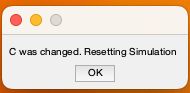
\includegraphics[width=5cm]{graphics/visualisation/dialog_cchange}
     \caption{Dialog showing the user that a change in $C$ was detected}
\end{figure}

\subsubsection{Duration Slider} [description of feature]

\begin{figure}[H]
    \centering
   	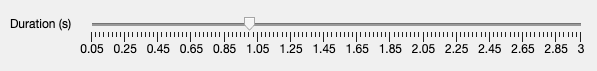
\includegraphics[width=\textwidth]{graphics/visualisation/ui_input_duration}
	\caption{Slider used to control the duration of the simulation}
\end{figure}

\subsubsection{Time Gauge} [description of feature]
\begin{figure}[H]
    \centering
   	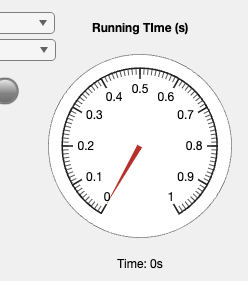
\includegraphics[width=5cm]{graphics/visualisation/ui_indicator_gage}
	\caption{Time gauge used to track the time progression of the simulation}
\end{figure}

\pagebreak
\subsection{Switching Operation}
EXPLAIN HERE
\begin{figure}[H]
    \centering
   	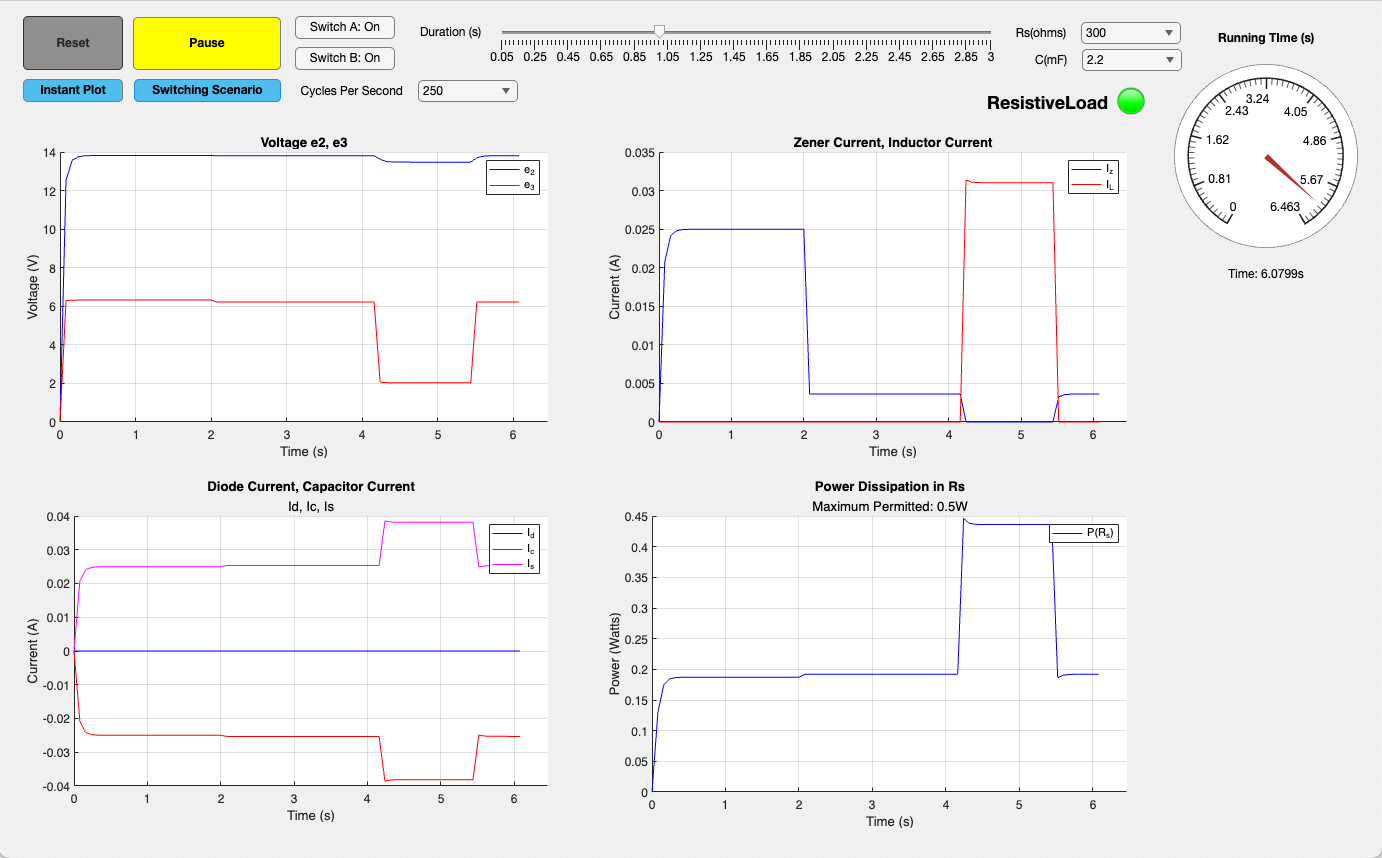
\includegraphics[width=\textwidth]{graphics/visualisation/switching_4}
	\caption{Slider used to control the duration of the simulation}
\end{figure}

\begin{lstlisting}[caption=Extract of code used to perform switching operation]
t1 = 2; % tn + t1=time when mode=ResistiveLoad
t2 = 2.2; % tn + t2= time when mode=Full load
t3 = 1.263; % time in full load
tend = t1 + t2 + t3 + 1; % total time (add 1s for steady state at end)
comp.t = 0:comp.TimeStep:tend; % Setup time vector

% Time breaks
resistiveLoadTime = t1;
fullLoadTime = t1+t2;
revertTime = fullLoadTime+t3;

for n=comp.k:length(comp.t)-1
if tn >= revertTime
  comp.mode = CircuitMode.ResistiveLoad;
elseif tn >= fullLoadTime
  comp.mode = CircuitMode.FullLoad;
elseif tn >= resistiveLoadTime
  comp.mode = CircuitMode.ResistiveLoad;
else
  comp.mode = CircuitMode.NoLoad;
end
	
tn_1 = tn + comp.TimeStep;
tn_2 = tn + comp.TimeStep / 2;
vin = comp.v([tn, tn_1, tn_2]); % Input voltage is a vector
y = powerSupply(comp.mode,vin,h,comp.ic,comp.C,comp.Rs);  % Perform iteration
    
% Plot y-values....
end
\end{lstlisting}
